% This file is for chapter 2

\chapter{Is Algorithm Selection Worth It? \\ Comparing Selecting Single Algorithms and Parallel Execution}

The material of this chapter is based on the following publication: 

H. Kashgarani and L. Kotthoff, “Is algorithm selection worth it? comparing selecting
single algorithms and parallel execution,” in \textit{AAAI Workshop on Meta-Learning and
MetaDL Challenge}, vol. 140 of \textit{Proceedings of Machine Learning Research}, pp. 58–64,
PMLR, 2021.


This chapter provides an empirical evaluation of SAT18-EXP solver performance (from the SAT Competition 2018) when running in parallel with other solvers at different levels of parallelism. Using the collected data, we trained two performance models based on the solver's sequential performance data and instance features. We then performed algorithm selection using these selectors to choose the best-predicted solver for each instance, comparing these results to running multiple solvers in parallel. The findings showed that algorithm selection is superior when many solvers run in parallel. The results in this chapter offer preliminary insights for this dissertation, highlighting the importance of selecting an instance-based subportfolio of solvers since, with fewer solvers, the overhead is minimal. The instance based subportfolio approach will be further developed in Chapter 4 and explored with variations in Chapter 5 and 6. 

\section{Abstract}
   For many practical problems, there is more than one algorithm or approach to solve them. Such algorithms often have complementary performance -- where one fails, another performs well, and vice versa. Per-instance algorithm selection leverages this by employing portfolios of complementary algorithms to solve sets of difficult problems, choosing the most appropriate algorithm for each problem instance. However, this requires complex models to effect this selection and introduces overhead to compute the data needed for those models. On the other hand, even basic hardware is more than capable of running several algorithms in parallel. We investigate the tradeoff between selecting a single algorithm and running multiple in parallel and incurring a slowdown because of contention for shared resources. Our results indicate that algorithm selection is worth it, especially for large portfolios.

\section{Introduction}

The performance of algorithms can vary significantly on different problem
instances and there is no single algorithm that performs well in all cases.
We can take advantage of such performance differences and create
algorithm portfolios to combine the complementary strengths of different
algorithms \cite{GOMES200143}. From this portfolio, we can choose the algorithm with the best performance for each problem instance -- this is known as the algorithm selection problem \cite{Rice1976}. This is usually done by using machine learning methods and features extracted from the instances \cite{Kotthoff2014}. Like all machine learning models, such approaches to algorithm selection make mistakes and in some cases choose an algorithm that does not have optimal performance. We can avoid this by exploiting modern multi-core architectures and simply running all algorithms in the portfolio in parallel, see e.g. \cite{sunnycp2}. While in theory optimal in terms of achieved performance, in practice contention for shared resources such as memory
and caches reduces overall performance.

We present, to the best of our knowledge, the first investigation into the
practical implications of running a large number of algorithms in parallel. We show the trade-off between algorithm selection that chooses a single algorithm and exploiting parallel resources and demonstrate that simply running all algorithms in a portfolio in parallel is not a panacea.

\section{Background}

Algorithm selection and other portfolio-based approaches have been applied in many areas of AI to improve performance. The first paper to introduce portfolios for solving hard AI problem considered a relatively simple parallel approach that executes all algorithms in the portfolio at the same time and stops them all as soon as the solution has been found by one \cite{Huberman1997}. \cite{GOMES200143,Hamadi2009} evaluate this strategy for stochastic algorithms and demonstrate that the variance of the time required to solve a problem decreases as the number of parallel runs increases.

This led to further approaches that take advantage of parallel processing by having several algorithms work independently or in cooperation on a given problem instance. \cite{Yun} construct algorithm portfolios for constraint satisfaction problems that are executed in parallel and show performance improvements for up to 16 processors, and \cite{sunnycp2} propose parallel portfolios with a dynamic schedule for up to 8 cores. Similarly, \cite{10.5555/1661445.1661516} show that by splitting the search space into sub-spaces, constraint solving portfolio approaches can take advantage of as many as 128 processors to achieve performance improvements.

For the Boolean satisfiability problem (SAT), simple static hand-crafted
parallel portfolios have been studied by \cite{roussel2012} and
\cite{wotzlawpfoliouzk} combined with a computed resource allocation for each solver. They employ a fixed selection of SAT solvers with good performance independently in parallel for a given number of cores.
\cite{gagliolo2006dynamic} introduce the dynamic algorithm portfolios that run a portfolio of algorithms with different shares of parallel processors along with an online time allocation learning approach. This includes a lifelong-learning approach in which the priority of algorithms is continually updated based on new runtime information.
\cite{petrik2006learning} also propose a method for enhancing
the performance of deterministic algorithms by running multiple algorithms in parallel for the same problem instance.  \cite{3s,Malitsky2012} propose a more sophisticated approach. They select algorithms through an improved k-nearest-neighbor approach and use both dynamic and static scheduling for multiple algorithms from the portfolio to improve the chance that a particular problem instance will be solved within a time limit.

Similarly, \cite{Marius2015} investigate parallel portfolio selection, and
\cite{aspeed} propose an approach to optimally schedule algorithms from a portfolio using answer set programming, while \cite{Gonard2019} take the simpler approach of running a small portfolio of algorithms in parallel for a short amount of time and using algorithm selection to tackle any problem instances that remain unsolved after that. To the best of our knowledge, all previous research has only simulated parallel execution without measuring the actual performance. We investigate the practical ramifications of running more than one algorithm in parallel.

\section{Experimental Setup}

We run algorithms sequentially and with varying degrees of parallelism. We build and evaluate algorithm selection models for sequential execution to be able to compare selecting a single algorithm to run multiple in parallel. We measure performance in terms of penalized average runtime with factor 10 (PAR10) and misclassification penalty (MCP). The PAR10 score is the observed performance unless an algorithm timed out on a particular instance, when the timeout multiplied by the penalization factor is assumed as the runtime. The misclassification penalty is the difference between the performance of the algorithm that was run and the optimal algorithm on the same instance, i.e. it
is always zero for the optimal algorithm.

We compare to the virtual best solver (VBS), which is the optimal algorithm from the portfolio for each problem instance to solve (cumulative misclassification penalty zero), and the single best solver (SBS), which is the algorithm from the portfolio with the best average performance across the entire set of problem instances to solve. The performance of the overhead-free parallel portfolio corresponds to the VBS.

We consider algorithms and problem instances from SAT, a popular application area for algorithm selection. We selected all 400 instances from the main track of the SAT Competition 2018 \cite{Heule2019} and computed their features using the SATzilla feature computation code \cite{satzilla}. We exclude 19 instances for which we were unable to extract features within two hours of computational time, for a total of 381 problem instances.

Our solvers also come from the main track of the 2018 SAT competition; we consider all 39 submitted solvers for a total of 14,859 algorithm runs. We use the same time limit as in the SAT competition; 5000 CPU seconds for solving a single instance. However, we allowed 128 GB of RAM; more than five times what was allowed in the competition. During the parallel runs, the total amount of memory is shared among all running algorithms. We run the algorithms sequentially, 10 in parallel, 20 in parallel, 30 in parallel, and 32 in parallel to fully saturate a machine with 32 cores.

We leverage the algorithm selection benchmark library ASlib \cite{BISCHL201641} and the LLAMA algorithm selection toolkit \cite{LLAMA} for our algorithm selection experiments. We build regression models that predict the performance of each algorithm in the portfolio individually and select the algorithm with the best-predicted performance, and pairwise regression models that predict the performance difference for each pair of algorithms and select
the algorithm with the aggregated best performance difference. We removed constant-valued (and therefore irrelevant) instance features and imputed missing feature values as the mean over all non-missing values of the feature.

For both regression and pairwise regression approaches, we use random forests as
the base machine learning models.
We tune their hyperparameters following
\cite{BISCHL201641}; we consider values of 10 to 200 for the \texttt{ntree}
hyperparameter and 1 to 30 for \texttt{mtry}. We optimize the hyperparameters
using random search with 250 iterations and perform a nested cross-validation
with 10 external and three internal folds to ensure unbiased performance
measurements. All other hyperparameters were left at their default values.

\begin{table*}[htb]
\centering
\begin{tabular}{l c c }
\toprule
\# parallel runs & \# timeouts & \# out of memory errors\\
\midrule
1 & 6982 (47\%) & 0 (0\%)\\
10 &  10281 (69.19\%) & 6 (0.04\%)\\
20 &  11853 (79.77\%) & 20 (0.13\%)\\
30 &  12590 (84.73\%) & 27 (0.18\%)\\
32 &  12715 (85.57\%) & 5 (0.03\%)\\
\bottomrule
\end{tabular}
\small \caption[Unsuccessful Runs for Each Level of Parallel Execution]{Unsuccessful runs for each level of parallel execution. The numbers in parentheses show the percentage of total runs that the number of unsuccessful runs corresponds to and are rounded to two decimal digits.}
\label{tab:errors}
\end{table*}

\section{Results}

\begin{table*}[htb]
\centering
\smallskip\begin{tabular}{l c c c c c} 
\toprule
metric & \# parallel runs & VBS & SBS & regression & pairwise regression\\
\midrule
PAR10 & 1 & 9256.089
 & 17585.66
 & 13004.31
 & 12588.44

 \\
& 10 & 13062.16
 & 27251.34
 & 19888.25
 & 20410.18

 \\
& 20 & 17099.23
 & 33630.54
 & 25233.38
 & 24970.07

 \\
& 30 & 19970.29
 & 36498.11
 & 28628.15
 & 27317.29

 \\
& 32 & 21674.1
 & 37285.5
 & 29937.23
 & 28888.24

\\ 
\midrule
MCP & 1 & 0 
& 1006.738 
& 441.0526 
& 379.5133
 \\
& 10 & 0 
& 1433.268 
& 684.2932 
& 733.7837
 \\
& 20 & 0 
& 1649.426 
& 811.264 
& 784.1721
 \\
& 30 & 0 
& 1645.936 
& 862.5388 
& 732.7824
 \\
& 32 & 0 
& 1556.284 
& 822.1427 
& 718.0386
\\
\bottomrule
\end{tabular}
\small \caption[PAR10 and MCP Performance Analysis: Comparing Algorithm Selection and Parallel Execution]{Performance in terms of PAR10 score and misclassification penalty for different numbers of algorithms run in parallel. The VBS is the performance of the parallel portfolio; SBS is shown for comparison. The ``regression'' and ``pairwise egression'' columns show the performance of the respective algorithm selection models.}
\label{tab:values}
\end{table*}

\begin{figure*}[htb]
    \setlength{\parindent}{0pt}
    \centering
    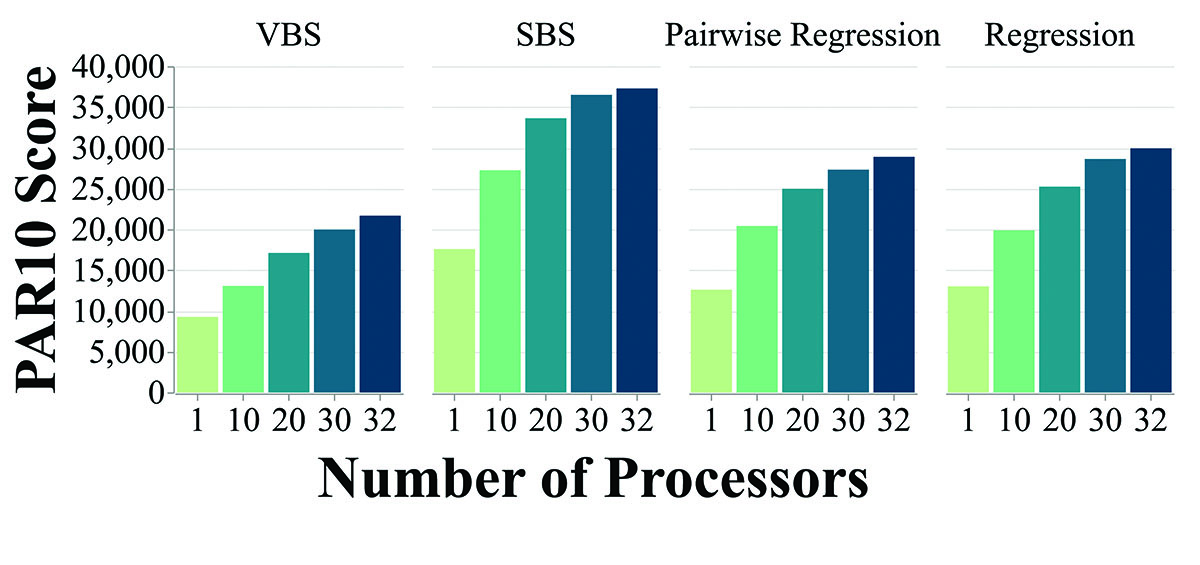
\includegraphics[width=0.48\linewidth]{PAR10}\\
    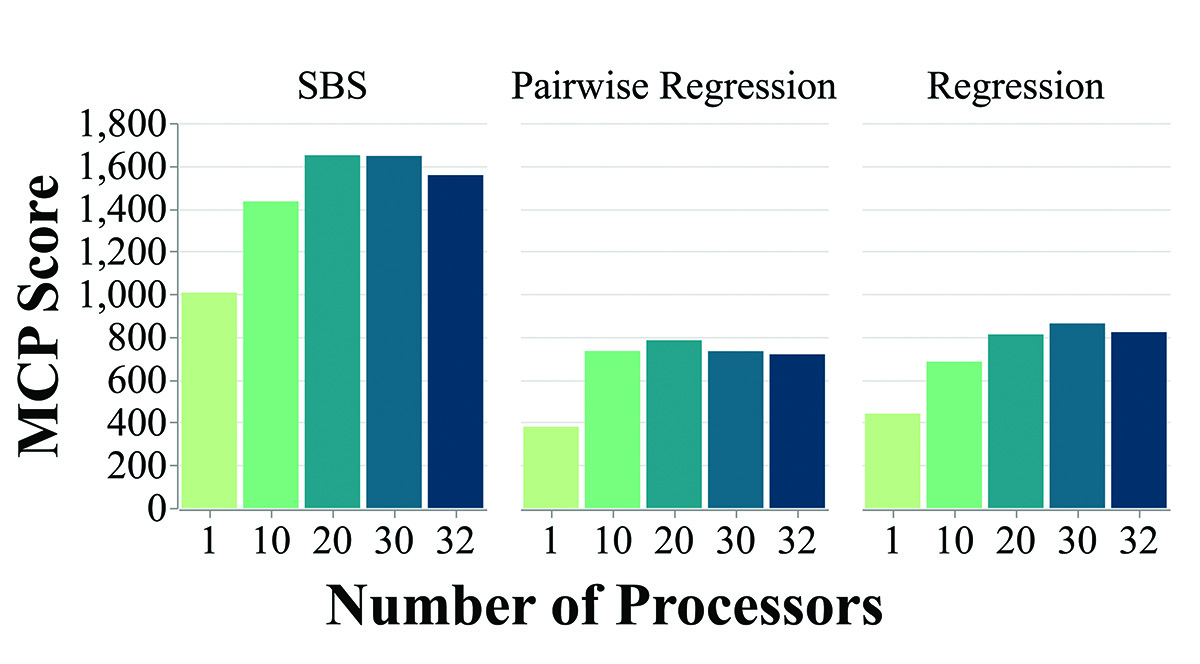
\includegraphics[width=0.48\linewidth]{MCP}
\small \caption[PAR10 and MCP Performance Analysis: Comparing Algorithm Selection and Parallel Execution]{Performance in terms of PAR10 score and misclassification penalty for different numbers of algorithms run in parallel. The VBS is the performance of the parallel portfolio; SBS is shown for comparison. The regression and pairwise regression bars show the performance of the respective algorithm selection models. We omit the plot for VBS performance in terms of MCP score as it is always zero by definition.}
    \label{fig:values}
\end{figure*}

We first evaluate the effect the number of parallel runs has on what fraction of all algorithm runs is successful. Table~\ref{tab:errors} shows the number and percentage of unsuccessful runs at each level of parallelism. With only one algorithm running at a time, 47\% of runs fail with a timeout. This increases as more and more algorithms are run in parallel. Similarly, the number of runs that fail because they run out of memory increases, as more and more runs share the same amount of physical memory. This does not significantly affect the results though, as even in the worst-case much less than 1\% of the total number of runs
is affected. Parallel runs have a much more significant effect on the number of timeouts though -- from 47\% runs that exceeded the available time when only a single algorithm is running at a time, we see an increase to 85.57\% of total runs when 32 algorithms are run in parallel. Altogether, 85.6\% of runs either time out or run out of memory when 32 algorithms are running in parallel; a significant increase over running only a single algorithm.

Table~\ref{tab:values} and Figure~\ref{fig:values} show the performance we
observed for all parallelism levels and approaches we consider. The PAR10 score
for the VBS increases significantly as we increase the number of algorithms run
in parallel; $\approx$41\% from one to 10 parallel runs. Similarly, the score
for the single best solver increases by $\approx$55\% for the same interval. The
PAR10 score is more than twice as high for 32 parallel runs compared to a single
run for both VBS and SBS -- contention for shared resources has a significant
impact on the time it takes to solve a set of instances. A large contributor to
the increase in PAR10 score is the increased number of unsuccessful runs because
of timeouts or memory outs.

We observe a similar decrease in performance as for the VBS and SBS for the algorithm selection approaches as the level of parallelism increases -- in fact, we observe even steeper performance losses in the beginning, with $\approx$53\% performance decrease from one algorithm to 10 for regression models and $\approx$62\% for pairwise regression models in terms of PAR10. However, we observe a performance increase for both approaches (lower MCP scores) when going from 30 algorithms run in parallel to 32, and a performance increase for pairwise regression model when going from 20 algorithms run in parallel to 30. It is unclear what exactly causes this performance increase; it is likely that the machine learning task that underlies the selection process becomes easier as more algorithms lose competitiveness because of timeouts and memory limits.


\begin{figure*}
    \setlength{\parindent}{0pt}
    \centering
    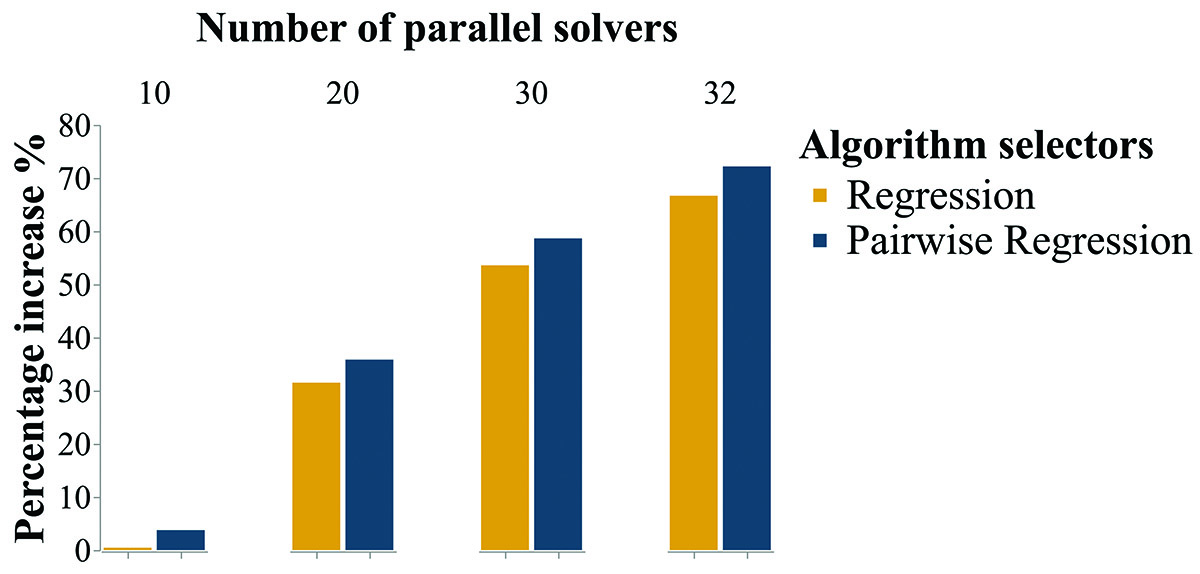
\includegraphics[width =.54\linewidth]{percentage}
    \small 
    \caption[PAR10 Score Increase with More Parallel Runs]{Percentage increase in terms of PAR10 score for running different numbers of algorithms in parallel compared to algorithm selector performance for choosing a single algorithm. For example, an increase of 100\% means that running the algorithms in parallel doubles the PAR10 score over selecting a single algorithm.}
    \label{fig:percentage}
\end{figure*}

Our results show that algorithm selection for choosing a single algorithm to run can beat parallel execution in practice for a large number of solvers. Figure~\ref{fig:percentage} shows that the performance of both the regression and pairwise regression algorithm selection approaches are better than the VBS for any level of parallelism beyond running a single algorithm. Both in terms of PAR10 and MCP, algorithm selection is always better than the single best solver. When using all 32 cores we have available, the VBS becomes more than 66\% worse than the regression algorithm selection approach and more than 72\% worse than
the pairwise regression algorithm selection approach. Even when running only 10 algorithms at the same time (and assuming that we know which 10 of the 39 total algorithms to run to maximize performance), the VBS is more than 0.4\% and 3\% worse than regression and pairwise regression approaches, respectively.

While the overhead-free parallel portfolio promises optimal performance, in theory, we clearly see that in practice this is not the case -- contention for shared resources and physical limits of the machine that is used to run the algorithms has a significant detrimental effect on performance. Even though algorithm selection models are not perfect, they outperform actual parallel portfolios in terms of observed performance even for a relatively small number of algorithms run in parallel.

\section{Conclusions and Future Work}

We investigated the actual observed performance of parallel
portfolios, in contrast to their theoretical performance that is usually used in the literature. We found that running even a relatively small number of
algorithms in parallel on the same machine can have a significant negative
impact on overall performance. Algorithm selection on the other hand chooses only a single algorithm and is able to achieve better overall performance, even though its predictions are not perfect and it does not always choose the algorithm with the best performance for solving a given problem instance.

An obvious avenue for future work is a hybrid approach to what we present here, where instead of a single algorithm several are chosen to run in parallel. Existing literature proposes a multitude of methods for doing so; however, none of these approaches have been evaluated as in the investigation we present here -- by actually running more than one algorithm in parallel and observing the performance rather than simulating this based on the performance observed when only a single algorithm is run at a time. In addition, there is scope for developing new approaches for dynamic resource allocation for algorithm selection.
% Cheat to bring in other references
\nocite{*} % delete or comment this out.
